\section{State rankings}

Using the statistical \& in/distinguishability graph methods described in \cref{sec:stats_methods}, we were able to develop both graph visualizations of state distinguishability and a possible ranking of the states.

\begin{figure}[h]
    \centering
    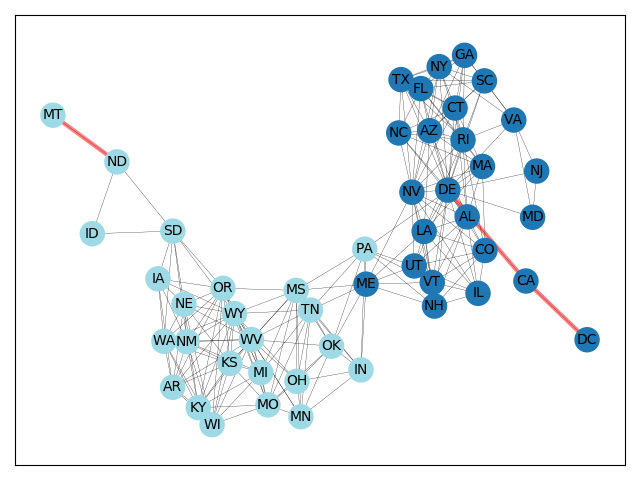
\includegraphics[width=0.85\textwidth]{caida/caida_network_invalid_comps.png}
    \repeatcaption{fig:caida_network_invalid_comps}{Indistinguishability graph of CAIDA+Atlas data as aggregated by state}
\end{figure}

\Cref{fig:caida_network_invalid_comps} shows an indistinguishability graph of comparisons between the states (previously seen in \cref{sec:stats_methods}), where node colors correspond to communities and bold red lines correspond to bridges.\footnote{You can think of bridges as indicators of comparison quality; any state on the end of a bridge can be compared to all but one of the other states.} As noted earlier, this graph has no disjoint subgraphs, so ranking by clusters is not possible. \Cref{fig:caida_network_valid_comps} shows the corresponding distinguishability graph, which is much more connected, indicating this data is a good candidate for the topological sort method.

\begin{figure}[h]
    \centering
    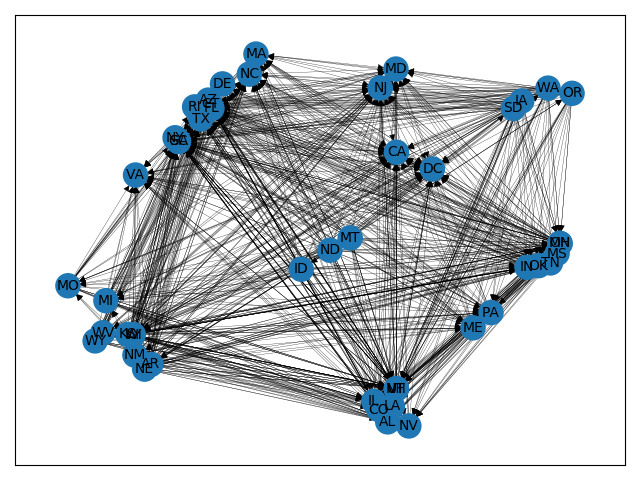
\includegraphics[width=0.85\textwidth]{caida/caida_network_valid_comps.png}
    \repeatcaption{fig:caida_network_valid_comps}{Distinguishability graph of CAIDA+Atlas data as aggregated by state}
\end{figure}

When sorted we obtain a list of 49 states (including the District of Columbia); two states were not reachable by a maximal topological sort. \ref{tab:caida_topological_state_rankings} shows this ranking, which roughly confirms what we'd expect based on prior notions and the heatmaps. States that are more populated or more urban are ranked higher than those are are less populated or more rural on average. The District of Columbia, being only a city and also the seat of the American federal government, naturally has the best internet. On the other hand, rural or more sparsely populated states like Montana or North Dakota rank at absolute last.

\begin{table}[h]
    \centering
    \begin{longtable}{ll|ll|ll|ll|ll}
        \textbf{Rank} & \textbf{State} & \textbf{Rank} & \textbf{State} & \textbf{Rank} & \textbf{State} & \textbf{Rank} & \textbf{State} & \textbf{Rank} & \textbf{State} \\
        \midrule
        \endhead
        \midrule
        \multicolumn{10}{r}{{Continued on next page}} \\
        \endfoot
        \endlastfoot
        \textbf{1 } & DC & \textbf{11} & TX & \textbf{21} &  LA & \textbf{31} & TN & \textbf{41} &    WY \\
        \textbf{2 } & DE & \textbf{12} & AL & \textbf{22} &  NV & \textbf{32} & MN & \textbf{42} &    NE \\
        \textbf{3 } & MD & \textbf{13} & CT & \textbf{23} &  PA & \textbf{33} & OH & \textbf{43} &    NM \\
        \textbf{4 } & CA & \textbf{14} & RI & \textbf{24} &  VT & \textbf{34} & WI & \textbf{44} &    OR \\
        \textbf{5 } & NJ & \textbf{15} & NC & \textbf{25} &  NH & \textbf{35} & KY & \textbf{45} &    IA \\
        \textbf{6 } & NY & \textbf{16} & MA & \textbf{26} &  UT & \textbf{36} & KS & \textbf{46} &    WA \\
        \textbf{7 } & SC & \textbf{17} & AZ & \textbf{27} &  IN & \textbf{37} & MO & \textbf{47} &    ID \\
        \textbf{8 } & GA & \textbf{18} & IL & \textbf{28} &  WV & \textbf{38} & MI & \textbf{48} &    MT \\
        \textbf{9 } & VA & \textbf{19} & CO & \textbf{29} &  MS & \textbf{39} & AR & \textbf{49} &    ND \\
        \textbf{10} & FL & \textbf{20} & ME & \textbf{30} &  OK & \textbf{40} & SD &             &       \\
        \caption{CAIDA+Atlas topologically sorted state rankings}
        \label{tab:caida_topological_state_rankings}
    \end{longtable}
\end{table}
